 \documentclass[paper=a4, DIV=13, BCOR=12mm, twoside=on, onecolumn=on, open = any, titlepage =on, parskip =half-, headsepline = on, footsepline = on, chapterprefix = on, sectionprefix = on, appendixprefix = off, fontsize = 11pt, numbers = noenddot, abstract = off]{scrreprt}
\usepackage[utf8]{inputenc}
\usepackage[ngerman]{babel}
\usepackage{amsmath}
\usepackage{amsthm}
\usepackage{amsfonts}
\usepackage{amssymb}
%\usepackage{makeidx}
\usepackage{graphicx}
\usepackage{tikz}
\usepackage{wrapfig}
%\usepackage{geometry}
\usepackage{parallel}
\usepackage{todonotes}
 \usepackage{mathptmx}
 \usepackage{pdfsync}
 \usepackage{url}
 \usepackage{float}
 \usepackage[linkbordercolor={1 1 1},urlbordercolor={1 1 1}] { hyperref}\urlstyle{rm}
 \usepackage[activate={true,nocompatibility},final,tracking=true,kerning=true,spacing=true]{microtype}
 \usepackage[section]{placeins}
 \usepackage{typearea}
\usepackage{chngcntr} 
\counterwithout{footnote}{chapter}

 %\usepackage[scaled=.90]{helvet}
 \usepackage[T1]{fontenc} 
%\newcommand{\changefont}[3]{ \fontfamily{#1} \fontseries{#2} \fontshape{#3} \selectfont}
%\changefont{cmr}{m}{n} %ppl for Palatino, ptm for Times New Roman
\setkomafont{title}{\rmfamily \bfseries}
\setkomafont{chapterentry}{\rmfamily \bfseries}
\setkomafont{chapter}{}
\usepackage{cutwin}
\usepackage[raggedleft]{titlesec}
%\titlelabel{\thetitle.\quad}
\titleformat*{\chapter}{\bfseries\small}
\titleformat*{\section}{\bfseries\normalsize}
\titleformat*{\subsection}{\bfseries \small}
\titleformat*{\subsubsection}{\bfseries \normalsize}

\usepackage{mwe}

\usepackage{xcolor}
\renewcommand*{\chapterformat}{%
  \thechapter\enskip
  \textcolor{gray!50}{\rule[-\dp\strutbox]{2pt}{\baselineskip}}\enskip
}
%\setkomafont{disposition}{\normalcolor\bfseries}


\hypersetup{
	pdftitle    = {},
	pdfsubject  = {Schritliche Arbeit zum Zweiten Staatsexamen},
	pdfauthor   = {Pamina Maria Berg},
	pdfkeywords = {} ,
	pdfcreator  = {pdfLatex},
	pdfproducer = {LaTeX with hyperref}
}







\setcounter{tocdepth}{2}

\usepackage{blindtext}
\usepackage{todonotes}
\usepackage{titlesec, blindtext, color}
\usepackage{setspace}
\usepackage{ragged2e}

\begin{document}
\newpage
\thispagestyle{plain}

\pagenumbering{Roman}



\begin{titlepage}
%\KOMAoptions{DIV=11, twoside}
\enlargethispage{\baselineskip}
%\begin{figure}[htbp]
%		\begin{minipage}[b]{25mm}
%			
\includegraphics[width=25mm,clip]{images/logo_uhh}
%		\end{minipage}
%		\begin{minipage}[b]{2mm}
%			
\includegraphics[width=1mm,height=25mm]{images/greypixel}
%		\end{minipage}
%		\begin{minipage}[b]{10cm}
%			{   
%				\vspace{2mm}
%				{\Large Universität Hamburg } \\
%				Fakultät für Mathematik,\\
%				Informatik und Naturwissenschaften \\
%				Department Informatik \\
%			}
%		\end{minipage}
%	\end{figure}

\vspace*{15ex} 
\begin{tabular}{c}

 \\
 \Large\textsc{Objektorientierte Programmierung}\\
\Large\textsc{in der Sekundarstufe II des Gymnasiums} \\
\tiny \\
\normalsize\textsc{Reflexion über Herangehensweisen}\\
\normalsize\textsc{zur Vermittlung grundlegender Programmierparadigmen}\\		  
\\
\\
\\
\normalsize Schriftliche Arbeit zur Zweiten Staatsprüfung für das Lehramt am Gymnasium \\
\normalsize im Fach Informatik\\
\\
\normalsize Hamburg, den 8.\,November\,2017

\end{tabular}

\vspace*{10ex}
	\noindent \textbf{Pamina Maria Berg}\\
	\noindent \rule{\textwidth}{0.4mm} 
	\noindent{\textrm{LiV}} \\	
	\noindent{\textrm{HS 16-08-Frö}}

\begin{tabbing}
\hspace{20em} \=  \kill
\emph{Erstgutachter} \> Sven Alisch \\
\emph{Zweitgutachterin} \> Christina von Bremen \\
 \> \\
\emph{Hauptseminarleitung} \> Dr. Sven Michael Fröhlich \\
\emph{Fachseminarleitung Informatik} \> Sven Alisch \\
\emph{Fachseminarleitung Mathematik} \> Hayo Zimmermann \\
 \> \\
 \hspace{20em} \=  \kill
\emph{Datum der mündlichen Prüfung} \> 21.12.2017 \\
 \hspace{10em} \=  \kill
\end{tabbing}

\end{titlepage}

\thispagestyle{empty}
\newpage
\thispagestyle{empty}

%\addchap*{Abstract}
%\onehalfspacing
%
%
%\addchap*{Zusammenfassung}
%\onehalfspacing
\definecolor{gray75}{gray}{0.75}
\newcommand{\hsp}{\hspace{20pt}}
\titleformat{\chapter}[hang]{\Large\bfseries}{\thechapter\hsp\textcolor{gray75}{|}\hsp}{0pt}{\Large\bfseries}

%\singlespacing
%\newpage
%\listoffigures
%\newpage
\tableofcontents
%\thispagestyle{empty}
\cleardoublepage
%\newpage
\pagenumbering{arabic}
\par \singlespacing
\renewcommand*{\dictumwidth}{.6667\textwidth}
\chapter{Einleitung}
\label{sec:einleitung}
\onehalfspacing

\dictum[Hans Aebli]{\justifying {"`Man kann sich Vorstellungen und Begriffe nicht in fertiger Form einverleiben. Man muss sie nachschaffen, nachkonstruieren."'}}

Die Lehre des Programmierens ist stark von einem schrittweisen Abarbeiten von Programmierparadigmen in einer ausgewählten Programmiersprache geprägt. In Lehrbüchern werden beispielsweise anhand von Projekten die klassischen Begriffe der Objektorientierung \emph{Klasse, Objekt, Methode, Parameter} vor- und zum Durcharbeiten am Computer bereitgestellt.

Informatische (Grund-)Bildung sollte als Teil der Allgemeinbildung (\todo{Zitat Breier 1994 raussuchen}) auch allgemeine Konzepte der Informatik vermitteln. \textsc{Hubwieser} weist in seinem Standardwerk zur Informatik-Didaktik auf einen leider immer noch auftretenden Sachverhalt hin:
\begin{quote}
Beim Betrachten entsprechender Rahmenpläne entsteht der Eindruck, dass entweder produktbezogene Anwenderschulungen oder Programmierkurse im Kleinen in diesem Unterricht durchgefuührt werden. (\cite[S.40]{hubwieser:07} aus \cite{koerber:93})
\end{quote}


\newpage
\par\singlespacing
\chapter{Ausgangssituation}
Es werden nun zunächst die systemischen Rahmenbedingungen, sowie die Voraussetzungen, die sich aus den inhaltlichen Lernzielen und den Lerngruppen ergeben, dargestellt.
\par\singlespacing
\section{Systemische Rahmenbedigungen}
\onehalfspacing
Der Unterrichtsplanung zugrunde liegen zum einen der Rahmenplan Informatik für die Gymnasiale Oberstufe (Vgl. \cite{oberstufe:09}) sowie das schulinterne Curriculum des Gymnasium Ohmoor. Im folgenden werden die für die durchgeführte Unterrichtspraxis relevanten Inhalte kurz erläutert.
\subsection{Rahmenplan}
Der Rahmenplan Informatik für die Gymnasiale Oberstufe in Hamburg spezifiziert die \textit{Objektorientierte Modellierung} als verbindlichen Inhalt, wobei eine explizite Forderung nach der "`Erarbeitung der Sprachelemente der verwendeten objektorientierten Programmiersprache"' (\cite[S. 17]{oberstufe:09}) besteht. Des weiteren sind verschiedene Anforderungsbereiche definiert, durch die sowohl fachliche als auch überfachliche Kompetenzen erworben und überprüft werden sollen. Der für die zu untersuchende Unterrichtssituation relevante Kompetenz bezieht sich auf den Bereich des \textit{Darstellen und Interpretieren}, in dem die Schülerinnen und Schüler "`Modelle und Algorithmen sowohl grafisch als auch verbal"' beschreiben können sollen (Vgl. \cite[S.16]{oberstufe:09}). Ein großer Fokus wurde planungsbedingt auch auf die Kompetenz des \textit{Kommunizieren und Kooperieren} gelegt (siehe hierzu Abschnitt \textbf{\ref{sec:vorgehensweisen}}).

\par \singlespacing
\subsection{Curriculum des Gymnasium Ohmoor}
\onehalfspacing
Die Fachschaft Informatik des Gymnasium Ohmoor konkretisiert im Schulinternen Curriculum die allgemein formulierten Vorgaben aus dem Rahmenplan Informatik. So ist im zweiten Semester der Gymnasialen Oberstufe das Thema \textit{Objektorientierte Modellierung/Programmierung von Grafiksystemen mit Java} angesiedelt (Vgl. \cite[S.6f.]{ohmoor:16}). Als verbindlicher Inhalt ist hier unter anderem die "`Erarbeitung von Sprachelementen: [...] Kontrollstrukturen"' (\cite[S.7]{ohmoor:16}) genannt, zu denen auch das Programmierparadigma der Schleifenkonstrukte gehört.

\par \singlespacing
 \section{Inhaltliche Ziele}
\onehalfspacing
Die inhaltlichen Ziele der Unterrichteinheit waren sowohl fachlicher als auch überfachlicher Art und lassen sich wie folgt zusammenfassen:
\begin{itemize}
\item Die SuS analysieren das BlueJ-Projekt, um sich mit den wesentlichen Merkmalen von Schleifen als Kontrollstrukturen in der Programmierung vertraut zu machen.
\item Die SuS erläutern anhand eines Minimalbeispiels in Java-Syntax den Ablauf einer \emph{for-, while-} oder \emph{do-while-}Schleife, indem sie eine Kurz-Vorführung im Plenum vorbereiten und durchführen.
\end{itemize}
Die hierzu passenden Einzellernziele sind:
\begin{itemize}
\item Die SuS geben mindestens die prägnanten Merkmale des Quellcodes an und beschreiben den grundsätzlichen Programmablauf im BlueJ-Projekt und sind bestenfalls in der Lage, eigene Schleifenkonstrukte zu implementieren und die Geeignetheit des gewählten Konstrukts zu begründen.
\item Die SuS beschreiben mindestens umgangssprachlich den Zusammenhang zwischen dem von ihnen gewählten Schleifenkonstrukt und ihrer Präsentation und beurteilen bestenfalls die Passung von Präsentation und Schleifenkonstrukt der eigenen und anderen Gruppen.
\item Die SuS stellen mindestens auf Nachfrage die wesentlichen Unterschiede der drei Schleifenkonstrukte dar und vergleichen diese bestenfalls im Hinblick auf verschiedene Einsatzszenarien.
\end{itemize}


\par \singlespacing
 \section{Lerngruppen}
\onehalfspacing
Der in dieser Arbeit untersuchte Lerngegenstand wurde in zwei Vergleichsgruppen mit methodisch variierten Vorgehensweisen unterrichtet. Diese werden im Folgenden als Vergleichsgruppe \textsc{\textbf{A}} und \textsc{\textbf{B}} bezeichnet.


Vergleichsgruppe \textsc{\textbf{A}}:\\
Der Informatik-Wahlpflichtkurs auf grundlegendem Niveau umfasst insgesamt 17 Schülerinnen und Schüler, davon sind vier weiblich und dreizehn männlich. Der Unterricht findet regelhaft donnerstags von 8:00 Uhr bis 9:30 Uhr statt. 
Es handelt sich um einen motivierten, kleinen Kurs, den ich zum zweiten Halbjahr übernommen habe. Die Leistungsspanne ist relativ groß, was sich in der kürzlich geschriebenen Klausur gezeigt hat – jedoch befindet sich die Mehrheit der SuS im oberen Leistungsdrittel. Einige SuS sind sehr programmieraffin und probieren eigenständig programmiertechnische Verfahren im Unterricht aus, die über das geforderte Maß hinausgehen. Schwächeren SuS fällt das Programmieren an sich noch etwas schwerer. Einer der SuS setzt sich leistungstechnisch deutlich von der Gruppe ab, da er durch sein Praktikum bereits umfassende Programmierkenntnisse in Java besitzt und diese selbstständig und mühelos im Unterricht umsetzen kann. Auch nimmt er immer wieder die Rolle eines Lernberaters ein und hilft seinen MitschülerInnen bei Schwierigkeiten. Bei Nachfragen antwortet er umfassend und adressatengerecht.\todo{Nochmal umformulieren, da zu nah an U-Entwürfen!!!}

Vergleichsgruppe \textsc{\textbf{B}}:\\
\todo{Beschreibung des PGW-Profil-Kurses}
Die erste Vergleichsgruppe ist der PGW-Profil-Kurs, bestehend aus 26 Schülerinnen und Schülern, deren Leistungsniveau sich eher heterogen gestaltet, wobei sich im Vergleich zu Gruppe \textsc{\textbf{B}} keine echte Leistungsspitze abzeichnet. Das Vorwissen der SuS in Bezug auf die zu untersuchende Unterrichtseinheit war (bedingt durch verschiedene Projektphasen der SuS in anderen Fächern) etwas geringer als bei der Vergleichsgruppe \textsc{\textbf{A}}, jedoch nicht in diesem Maße, als dass eine Lernhürde bei der Analyse von Quelltext zu erwarten gewesen wäre. 

Beide Vergleichsgruppen waren bereits sicher im Umgang mit der Entwicklungsumgebung \emph{BlueJ} und hatten in unterschiedlichen Kontexten eigene Programmiererfahrungen mit Java machen können.

\chapter{Die Praxissituation}
\onehalfspacing
 Im folgenden werden die für die Planung der Praxissituation maßgeblichen Details und Entscheidungen, sowie die Vorgehensweisen für die Durchführung beschrieben. Es wird zunächst eine kurze Information 
\par \singlespacing
 \section{BlueJ}
\onehalfspacing
\todo{Hier wäre noch Spielraum...}
\label{sec:bluej}
Die Java-Entwicklungsumgebung BlueJ wurde an der Monash University in Australien mit dem Ziel entwickelt, eine Umgebung für Programmieranfänger mit einer einfachen Benutzerschnittstelle zu schaffen (Vgl. \cite[S.14]{barnes:03}). \textsc{Barnes} und \textsc{Kölling} betonen die besondere Geeignetheit von BlueJ in der Lehre und führen diese auf die native Visualisierung der Klassenstruktur und die damit einhergehende Möglichkeit, mit den Objekten direkt zu interagieren, "`ohne Testklassen schreiben zu müssen"' (Vgl. \cite[S.15]{barnes:03}). 

%Es handelt sich jedoch bei der Entwicklung objektorientierter Programme mit BlueJ keinesfalls um die Benutzung einer reduzierten Version von Java. BlueJ läuft, wie andere Entwicklungsumgebungen, auf dem aktuellen Java Development Kit (JDK). Auch als Compiler und virtuelle Maschine (JVM) wird Software der Firma Oracle (bis 2010 Sun Microsystems) verwendet (Vgl. \cite[S.15]{barnes:03}).

%\begin{figure}[htb]
%\centering
%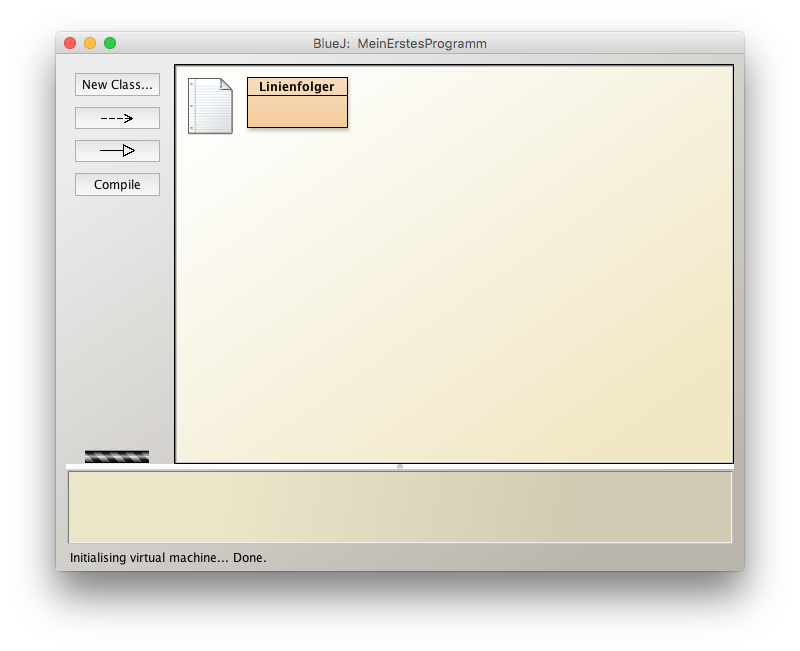
\includegraphics[scale=0.3]{images/firstprogram.png} 
%\caption{Die Benutzeroberfläche von BlueJ}
%\label{fig:BlueJ UI}
%\end{figure}
%\todo{anderes Bild einfügen}
%Inzwischen wird nicht nur in den Universitäten BlueJ als Werkzeug zur Einführung in die Programmiersprache Java und die objektorientierte Programmierung genutzt. Auch im Schulkontext hat die intuitive Bedienung und übersichtliche Gestaltung Anklang gefunden, da BlueJ "`eine einfache Entwurfssicht für die Analyse gegebener Lösungen und für die Planung neuer Lösungen"' \cite[S.6]{ehmann:09} zur Verfügung stellt. Eine weitere Besonderheit besteht darin, dass -- im Gegensatz zu den meisten anderen Entwicklungsumgebungen -- in BlueJ "`schnell einige Objekte erzeugt und sofort untersucht werden [können]"' \cite[S.6]{ehmann:09}. Hierzu bietet BlueJ die \emph{Inspect-}Funktion an, die über das Kontextmenü eines erzeugten Objekts erreichbar ist und die Werte der Feldvariablen genau dieses Exemplars einer Klasse anzeigt.

\par \singlespacing
 \section{Bausteine der Unterrichtsplanung und Didaktische Entscheidungen}
\onehalfspacing

Die Unterrichtseinheit zum Lerngegenstand Schleifenkonstrukte besteht aus zwei Bausteinen, die inhaltlich ineinandergreifen, jedoch methodisch andere lerntheoretische Ansätze verfolgen. 

Der erste Baustein besteht aus einem BlueJ-Projekt, welches ich durch meine Tätigkeit als Übungsgruppenbetreuerin an der Universität Hamburg kennengelernt habe. Dieses Projekt ist an das Lehrbuch zur Objektorientierten Programmierung mit Java und BlueJ von \textsc{Barnes} und \textsc{Kölling} angelehnt und versucht, über kurze Methodenrümpfe, die von den Lernenden analysiert werden sollen, verschiedene Arten von Schleifenkonstrukten zu vermitteln.\\
Zusätzlich zu diesem Kurzprojekt haben die SuS ein Arbeitsblatt mit verschiedenen Aufträgen bekommen, welche sie schrittweise durch das Projekt führen sollten (Vgl. Anhang \textbf{A}).

Betrachtet man die Arbeitsaufträge, so sieht man, dass die spezifischen Vorteile von BlueJ genutzt werden, um die SuS mit dem Quellcode interagieren zu lassen: Sie sollen verschiedene Beispiele ausführen und dabei auf die jeweiligen Rückgaben des Programms achten. Die SuS werden demnach aufgefordert, die informatischen Vorgänge zu \emph{beobachten} (s. hierzu auch \cite[S.67ff.]{aebli:11}). 

Den zweiten Baustein haben sich die SuS jeweils eigenständig erarbeitet: Auf Grundlage ihrer basalen Syntaxkenntnisse haben die SuS in Gruppen verschiedene "`leere"' Schleifenkonstrukte in Java bekommen, deren Ablauf sie jeweils zunächst analysieren und dann in Form einer interaktiven Gruppenpräsentation darstellen sollten. Hierbei war es den SuS freigestellt, welche Hilfmittel sie dazu einsetzen und welche Aktivitäten vorgeführt werden können. Es sollte lediglich deutlich werden, wie die von ihnen vorgestellte Sequenz von Anweisungen mit der von ihnen ausgewählten \emph{for-, while-} oder \emph{do-while-}Schleife im Zusammenhang steht.

\par \singlespacing
 \section{Vorgehensweisen und Methodische Entscheidungen}
 \label{sec:vorgehensweisen}
\onehalfspacing

Die beiden Bausteine wurden zum Zweck eines produktiven Vergleichs in jeweils umgekehrter Reihenfolge mit den Vergleichsgruppen durchgeführt. So hat Vergleichsgruppe \textsc{\textbf{A}} zunächst mit der interaktiven Vorführung, also dem enaktiven Ansatz, begonnen und sich danach mit dem BlueJ-Projekt beschäftigt -- der Vergleichsgruppe \textsc{\textbf{B}} wurde zuerst der Quelltext und das Arbeitsblatt ausgegeben, mit deren Erarbeitung sie in Partnerarbeit und ohne weitere Einhilfen beauftragt wurden \todo{unschöne Formulierung}.

\par \singlespacing
\chapter{Reflexion der Herangehensweisen}
\onehalfspacing
 Bei der Reflexion der Herangehensweisen und der Praxissituationen wird es nun darum gehen, die beiden in ihrer Reihenfolge variierten Vorgehensweisen kritisch zu betrachten, in Bezug zueinander zu setzen und eine daraus resultierende Fragestellung zu entwickeln und untersuchen.

\par \singlespacing
\section{Kritische Betrachtung}
\onehalfspacing

- Lernhürden bei Start mit Programmierung aufgetreten\\
- Enaktiver Asnatz bietet viel Spielraum für sehr spezifische Randfälle\\
- EA fördert kreativen Umgang und Durcharbeiten von trockener Syntax\\
- Bei Vorstellung des EA durch SUS direkte Diskussionsmöglichkeiten -> Mehr Zeit für den Vergleich der Lösungen einplanen, um tieferes Verständnis zu fördern\\
- Reihenfolge (Präferenz) stark v individ. SuS abhängig\\
- EA von allen SuS als förderlich wahrgenommen\\
- PA setzt Syntaxkenntnisse voraus\\
- vorgegebene Konstrukte müssen analysiert und verstanden werden\\


\par \singlespacing
 \section{Resultierende Fragestellung}
\onehalfspacing

Fällt der Umgang mit Programmiersprachen und -konzepten leichter, wenn neben der theoretischen Vermittlung auch eine Handlungsorientierung abseits des Computers stattfindet?

\par \singlespacing
\chapter{Alternativkonzeption}
\onehalfspacing

Aufgrund der Untersuchung und Reflexion der Praxissituation werden die daraus resultierenden Konsequenzen und Fragestellungen nun in einer Alternativkonzeption der Unterrichtsstunde zum Einen und mithilfe von Schlussfolgerungen für die gesamte Unterrichtseinheit der \emph{OOP/OOM} zum Anderen verarbeitet \todo{hier fehlt noch ein schöner Halbsatz}

- statt autodidaktisch v. SuS beispielhaft gemeinsam im Vorwege oder verknüpft mit EA, so dass vorgegebene Schleifen nachgespielt werden sollen\\
- IDEE: Anknüpfen/Verknüpfen von EA mit Programmierprojekt\\
- Kontext Spiele/Möbelplaner -> Modellbildung auf Papier -> Ausschneiden, legen,...

\par \singlespacing
 \section{Vermittlung des beschriebenen Programmierparadigmas}
\onehalfspacing



\par \singlespacing
 \section{Schlussfolgerungen für die Unterrichtseinheit}
\onehalfspacing

\newpage
\chapter{Fazit und Ausblick}
\onehalfspacing

\begin{figure}[htb]
\centering
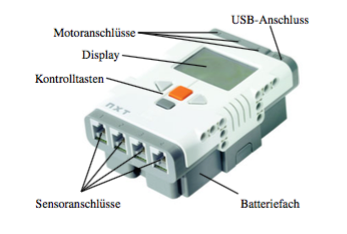
\includegraphics[scale=0.7]{images/NXT-Stein.png} 
\caption[Der NXT-Stein]{Der NXT-Stein \cite[S. 42]{berns:10}}
\label{fig:NXT Stein}
\end{figure}

\begin{figure}[htb]
\centering
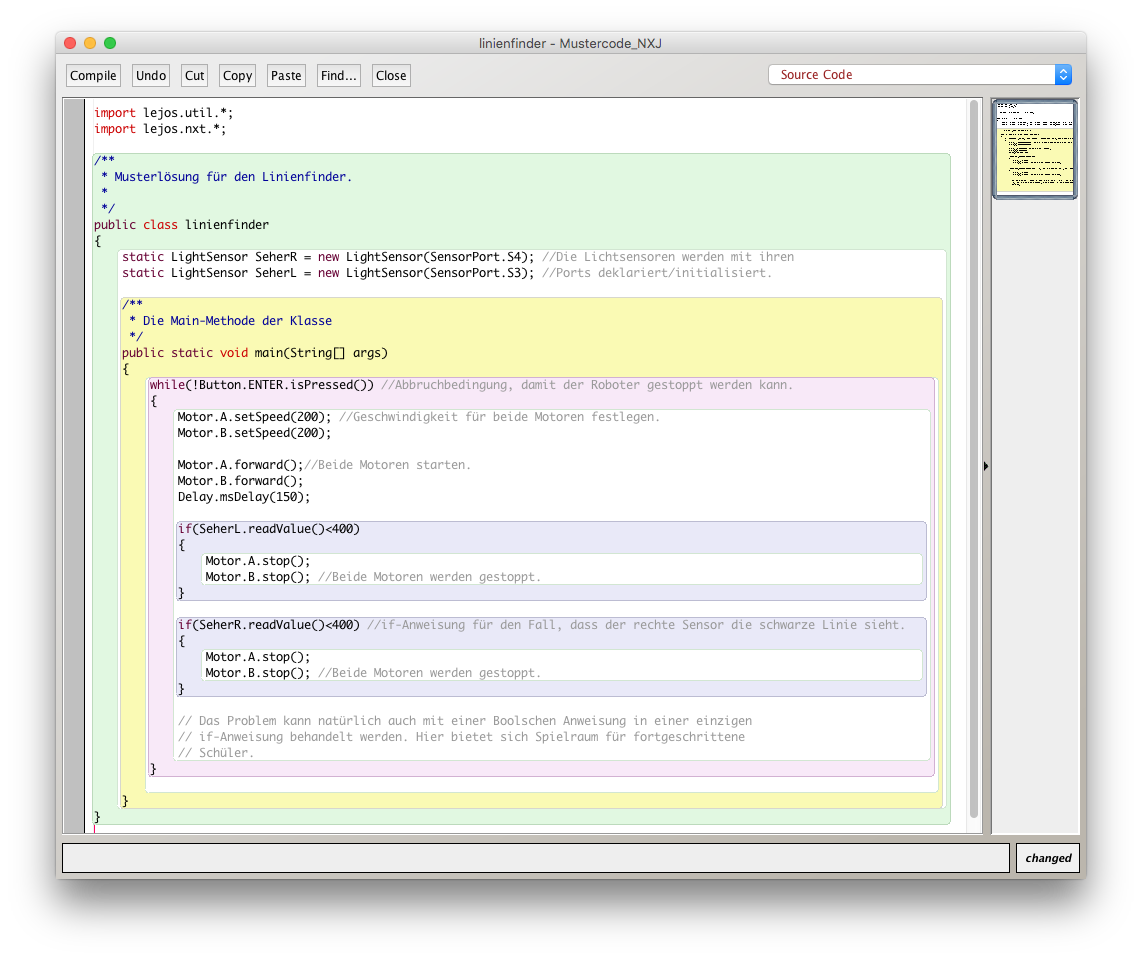
\includegraphics[width=\textwidth]{images/linienfinder_bluej.png} 
\caption{BlueJ-Beispiel zum Finden einer Linie}
\label{fig:Bsp BlueJ Linienfinder}
\end{figure}




\newpage
\begin{thebibliography}{ABCDEF}

\renewcommand{\refname}{\normalsize Literaturverzeichnis}

%\bibitem[Abe01]{abend:01}
%Michael Abend. "'Robotik und Sensorik. Darstellungsschwerpunkt: Selbständige Entwicklung "`unscharfer"' Algorithmen zur räumlichen Orientierung (unter Verwendung des LEGO-Mindstorms-Systems)", \emph{Schriftliche Prüfungsarbeit zur zweiten Staatsprüfung für das Amt des Studienrats}, Berlin, 2001

\bibitem[Abt15]{abts:15}
Dietmar Abts. \emph{Grundkurs JAVA. Von Grundlagen bis zu Datenbank- und Netzwerkanwendungen}, 8., überarbeitete und erweiterte Auflage, Springer Vieweg, Wiesbaden, 2015

\bibitem[Aeb11]{aebli:11}
Hans Aebli. \emph{Zwölf Grundformen des Lehrens. Eine Allgemeine Didaktik auf psychologischer GRundlage. Medien und Inhalte didaktischer Kommunikation, der Lernzyklus}, 14. Auflage, Klett-Cotta, Stuttgart, 2011

\bibitem[Bar03]{barnes:03}
David J. Barnes, Michael Kölling. \emph{Objektorientierte Programmierung mit Java. Eine praxisnahe Einführung mit BlueJ}, Übersetzt von Axel Schmolitzky, Pearson Studium, München, 2003

\bibitem[Bre94]{breier:94}
Norbert Breier. \emph{Informatische Bildung als Teil der Allgemeinbildung}, LOG IN 14, H. 5/6., 1994
%\pagebreak 

%\bibitem[Ber10]{berns:10}
%Karsten Berns, Daniel Schmidt. \emph{Programmierung mit LEGO MINDSTORMS NXT. Robotersysteme, Entwurfsmethodik, Algorithmen}, Springer Heidelberg Dordrecht London New York, 2010

%\bibitem[Bow12]{bowes:12}
%David Bowes. \url{http://homepages.herts.ac.uk/~comqdhb/lego/bluej.php}, Abgerufen am 07.02.2016, Herfortshire, 2012, Lejos NXJ extension for BlueJ

%\bibitem[BricxCC]{bricxcc}
%o.V. URL: \url{http://bricxcc.sourceforge.net/}, Abgerufen am 02.02.2016

\bibitem[Ehm09]{ehmann:09}
Matthias Ehmann et al. \emph{Duden Informatik - Sekundarstufe I / 9./10. Schuljahr - Objektorientierte Programmierung mit BlueJ}, Duden Schulbuchverlag Berlin Mannheim, 2009

\bibitem[GyOhm16]{ohmoor:16}
Fachschaft Informatik. \emph{Schulinternes Curriculum Informatik. Sekundarstufe II Wahlbereich und Profile}, Hamburg, Stand: 14.03.2016

%\bibitem[Her12]{hertzberg:12}
%Joachim Hertzberg, Kai Lingemann, Andreas Nüchter. \emph{Mobile Roboter. Eine Einführung aus Sicht der Informatik}, Springer-Verlag Berlin Heidelberg, 2012

\bibitem[HH09]{oberstufe:09}
Behörde für Schule und Berufsbildung Hamburg (Hrsg.). \emph{Informatik -- Bildungsplan  Gymnasiale Oberstufe}, Hamburg, 2009

\bibitem[HH11]{gymsek1:11}
Behörde für Schule und Berufsbildung Hamburg (Hrsg.). \emph{Informatik Wahlfplichtfach -- Bildungsplan Gymnasium Sekundarstufe I}, Hamburg, 2011

\bibitem[HH14]{stsmittel:14}
Behörde für Schule und Berufsbildung Hamburg (Hrsg.). \emph{Informatik Wahlpflichtfach -- Bildungsplan Stadtteilschule Jahrgangsstufen 7 -- 11}, Hamburg, 2014

\bibitem[Hub07]{hubwieser:07}
Peter Hubwieser. \emph{Didaktik der Informatik}, 3. Auflage, Springer-Verlag Berlin Heidelberg, 2007

\bibitem[Hum02]{humbert:02}
Ludger Humbert, Sigrid Schubert. \emph{Fachliche Orientierung des Informatikunterrichts in der Sekundarstufe II}, Didaktik der Informatik Universität Dortmund, Report Nr. 77, Februar 2002

\bibitem[Koe93]{koerber:93}
Koerber B., Peters I.R.: \emph{Informatikunterricht und informationstechnische Grundbildung –
ausgrenzen, abgrenzen oder integrieren?}, Troitzsch, S. 108--115, 1993 \todo{Vornamen der Autoren}

\bibitem[Mod11]{modrow:11}
Eckart Modrow. "{Visuelle Programmierung -- oder: Was lernt man aus Syntaxfehlern?}", In: Marco Thomas (Hrsg.): \emph{Informatik in Bildung und Beruf. 14. GI-Fachtagung "`Informatik und Schule – INFOS 2011"'}, S. 27--36, 2011

%\bibitem[Lego]{lego}
%o.V. URL: \url{http://www.lego.com/en-us/mindstorms/history}, Abgerufen am 06.11.2015, LEGO, 2015
%
%\bibitem[leJOS]{lejos}
%o.V. URL: \url{http://www.lejos.org/nxj.php}, Abgerufen am 14.12.2015, leJOS Java for Lego Mindstorms, 2015

%\bibitem[Lil08]{lilienthal:08}
%Carloa Lilienthal. "Komplexität von Softwarearchitekturen -- Stile und Strategien --", \emph{Dissertation im Fachbereich Informatik der Universität Hamburg}, Hamburg, 2008


%\bibitem[Sch04]{schreiber:04}
%Rafael Schreiber. "Der Einsatz von LEGO-Mindstorms im Informatikunterricht der 11. Klasse der Leonard-Bernstein-Oberschule. Sicherung und Transfer grundlegender algorithmischer Strukturen in NQC.", \emph{Schriftliche Prüfungsarbeit im Rahmen der zweiten Staatsprüfung für das Amt des Studienrats}, Berlin, 2004

\bibitem[Schwa07]{schwarzer:07}
Christine Schwarzer, Petra Buchwald. "{Umlernen und Dazulernen}.", In: Michael Göhlich, Christoph Wulf, Jörg Zirfas (Hrsg.): \emph{Pädagogische Theorien des Lernens}, Beltz, Weinheim und Basel,  S. 213--221, 2007


%\bibitem[RWTH]{rwth}
%o.V. URL:{http://schuelerlabor.informatik.rwth-aachen.de/simulator}, Abgerufen am 02.02.2016, Simulator für LEGO Mindstorms NXT Roboter

%\bibitem[Sto01]{stolt:01}
%Matthias Stolt. "Roboter im Informatikunterricht", 2001

\bibitem[Ull12]{ullenboom:12}
Christian Ullenboom. \emph{Java ist auch eine Insel -- Das umfassende Handbuch}, 10. Auflage, Galileo Press, Bonn, 2012

\bibitem[Wag05]{wagner:05}
Oliver Wagner. "LEGO Roboter im Informatikunterricht. Eine Untersuchung zum Einsatz des LEGO-Mindstorms-Systems zur Steigerung des Kooperationsvermögens im Informatikunterricht eines Grundkurses (12. Jahrgang, 2. Lernjahr) der Otto-Nagel-Oberschule (Gymnasium)", \emph{Schriftliche Prüfungsarbeit im Rahmen der zweiten Staatsprüfung für das Amt des Studienrats}, Berlin, 2005

%\bibitem[Zül90]{züllighoven:90}
%Reinhard Budde, Heinz Züllighoven. \emph{Software-Werkzeuge in einer Programmierwerkstatt. Ansätze eines hermeneutisch fundierten Werkzeug- und Maschinenbegriffs}, Oldenbourg, München [u.a.], 1990
\end{thebibliography}
\newpage

\KOMAoptions{headsepline=off}
%\KOMAoptions{footsepline=off}

\addsec*{Anhang A}
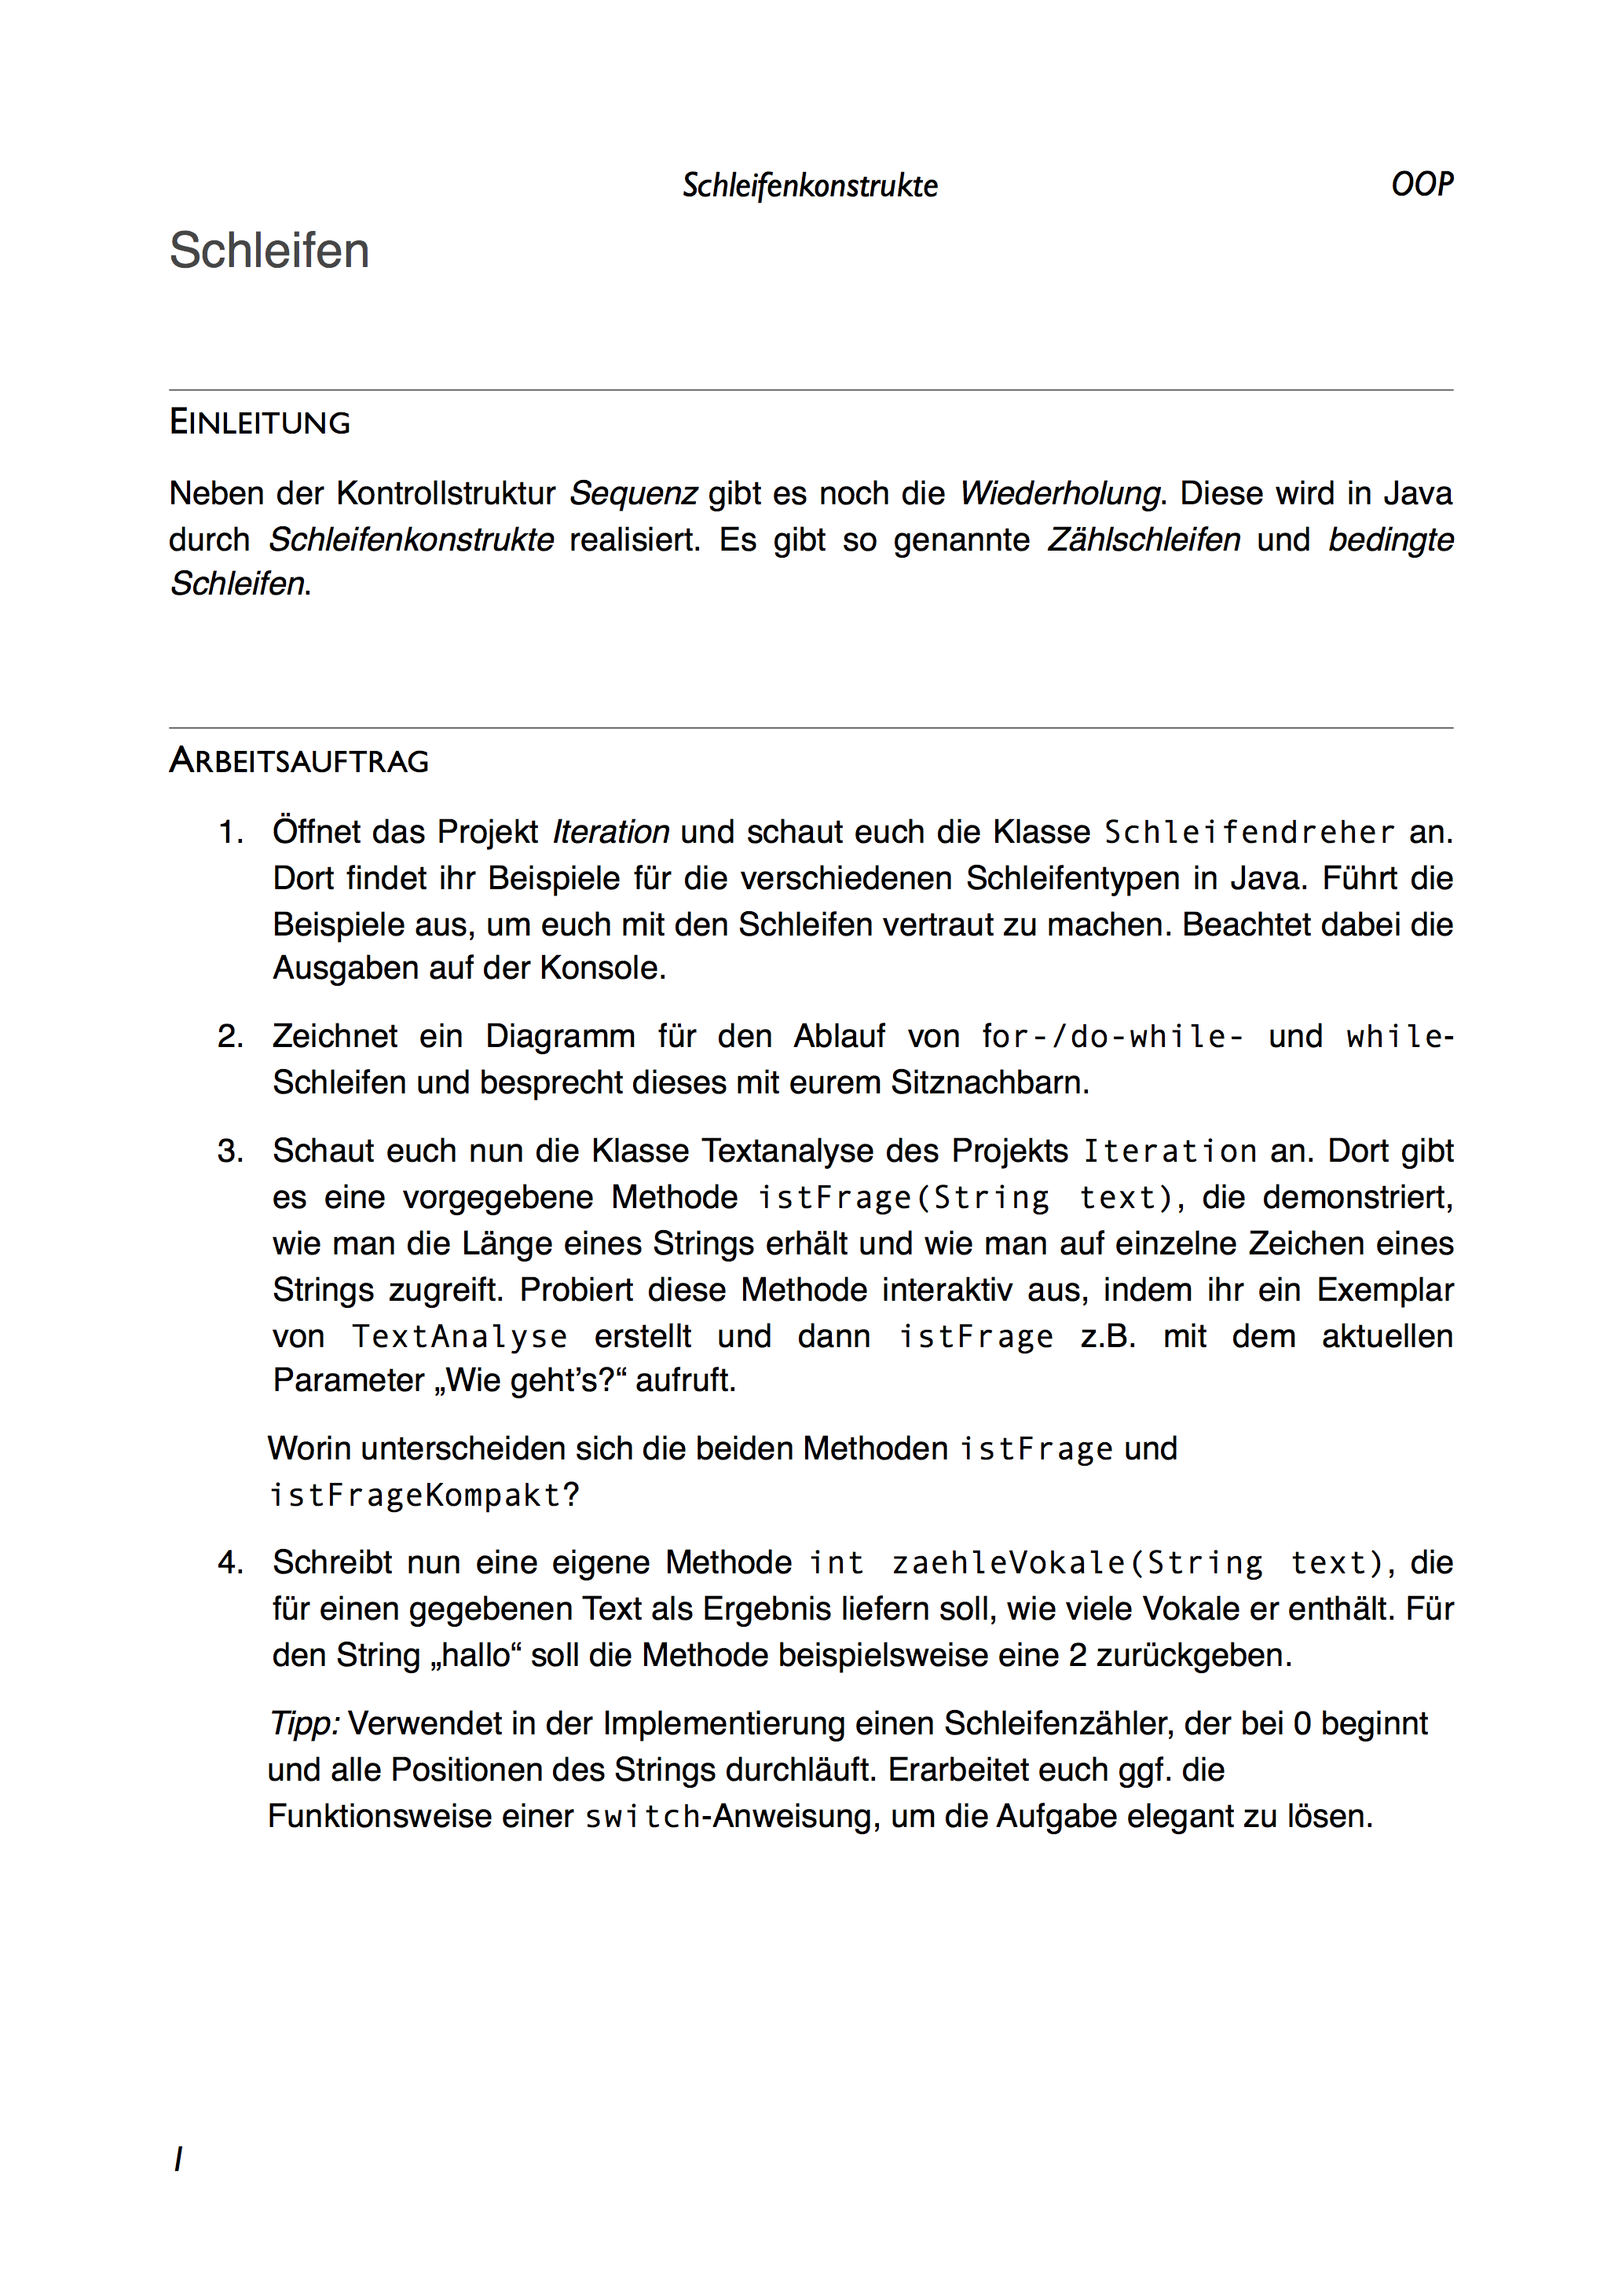
\includegraphics[height=\textheight]{images/AB_Schleifenkonstrukte.png}

\cleardoublepage
\newpage
\thispagestyle{empty}
\vspace*{\fill}
"Hiermit versichere ich an Eides statt, dass ich die Arbeit selbstständig verfasst und keine anderen als die angegebenen Hilfsmittel – insbesondere keine im Quellenverzeichnis nicht benannten Internet-Quellen – benutzt habe, die Arbeit vorher nicht in einem anderen Prüfungsverfahren eingereicht habe und die eingereichte schriftliche Fassung der auf dem elektronischen Speichermedium entspricht."\\

Hamburg, 8.\,März 2016 \hspace*{\fill} \dots \dots \dots \dots \dots \dots \dots \dots \dots\\
\hspace*{\fill} Pamina Maria Berg \quad $\,$
\end{document}